\let\negmedspace\undefined
\let\negthickspace\undefined
\documentclass[journal]{IEEEtran}
\usepackage[a5paper, margin=9mm, onecolumn]{geometry}
\usepackage{lmodern} 
\usepackage{tfrupee} 

\setlength{\headheight}{1cm} 
\setlength{\headsep}{0mm}     

\usepackage{gvv-book}
\usepackage{gvv}
\usepackage{cite}
\usepackage{amsmath,amssymb,amsfonts,amsthm}
\usepackage{algorithmic}
\usepackage{graphicx}
\usepackage{textcomp}
\usepackage{xcolor}
\usepackage{txfonts}
\usepackage{listings}
\usepackage{enumitem}
\usepackage{mathtools}
\usepackage{gensymb}
\usepackage{comment}
\usepackage{multicol}
\usepackage[breaklinks=true]{hyperref}
\usepackage{tkz-euclide} 
\usepackage{listing}

\graphicspath{ {./figs/} }

\begin{document}


\title{
ASSIGNMENT 2: GATE 2011 \\
IN:INSTRUMENTATION ENGINEERING}
\author{AI25BTECH11013-Gautham Pocha}
\maketitle
\renewcommand{\thefigure}{\theenumi}
\renewcommand{\thetable}{\theenumi}


\begin{enumerate}

\item The matrix $ \Vec{M} = \myvec{-2 & 2 & -3 \\ 2 & 1 & -6 \\ -1 & -2 & 0 } $ has eigenvalues -3, -3, 5. An eigenvector corresponding to the eigenvalue 5 is $\myvec{1\ 2\ -1}$. One of the eigenvectors of the matrix $ M^3 $ is
\begin{multicols}{4}
\begin{enumerate}
\item $\myvec{1\ 8\ -1}^T$
\item $\myvec{1\ 2\ -1}^T$
\item $\myvec{1\ 2\ -1}^T$
\item $\myvec{1\ 1\ -1}^T$
\end{enumerate}
\end{multicols} \hfill(GATE IN 2011)

\item The contour integral $ \oint_C e^\frac{1}{z} dz $, with $ C $ as the counter-clockwise unit circle in the $ z $-plane, is equal to
\begin{multicols}{4}
\begin{enumerate}
\item $0$
\item $2\pi$
\item $2\pi sqrt(-1)$
\item $\infty$
\end{enumerate}
\end{multicols} \hfill(GATE IN 2011)

\item Consider the signal $ x(t) = e^t,  t \geq 0; \quad x(t) = 0, t < 0 $. Let $ X(\omega) $ denote the Fourier transform of this signal. The integral $ \frac{1}{2\pi}\int_{-\infty}^{\infty} X(\omega) d\omega $ is
\begin{multicols}{4}
\begin{enumerate}
\item $0$
\item $1/2$
\item $1$
\item $\infty$
\end{enumerate}
\end{multicols} \hfill(GATE IN 2011)

\item The continuous-time signal $ x(t) = \sin(\omega_0 t) $ is periodic signalever, for its discrete-time counterpart $ x[n] = \sin(\omega_0 n) $ to be periodic, the necessary condition is
\begin{multicols}{2}
\begin{enumerate}
\item $0 \leq \omega_0 < 2\pi$
\item $ \frac{2\pi}{\omega_0} $ must be an integer
\item $ \frac{2\pi}{\omega_0} $ must be a rational number
\item none
\end{enumerate}
\end{multicols} \hfill(GATE IN 2011)

\item Consider a periodic signal $ x(t) $ 
\begin{figure}[H]
    \centering
      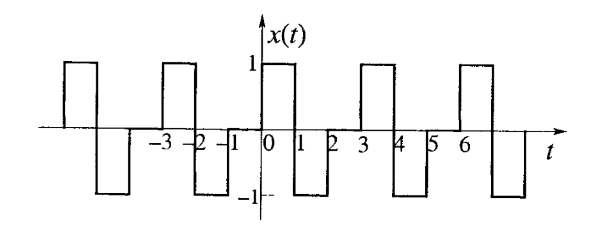
\includegraphics[width=0.6\textwidth]{1.png} 
      \caption{}
    \label{fig:fig1} 
\end{figure}
with Fourier series representation $ x(t) = \sum_{k=-\infty}^{\infty} a_k e^{j(2\pi/T)kt} $. Which one of the following statements is TRUE?
\begin{multicols}{2}
\begin{enumerate}
\item $ a_k = 0 $, for $ k $ odd integer and $ T = 3 $
\item $ a_k = 0 $, for $ k $ even integer and $ T = 3 $
\item $ a_k = 0 $, for $ k $ even integer and $ T = 6 $
\item $ a_k = 0 $, for $ k $ odd integer and $ T = 6 $
\end{enumerate}
\end{multicols} \hfill(GATE IN 2011)

\item The integral
$ \frac{1}{\sqrt{2\pi}} \int_{-\infty}^{\infty} t^2 e^{-t^2/2} \delta(1-2t) dt $ is equal to

\begin{multicols}{4}
\begin{enumerate}
\item $\frac{1}{8\sqrt{2\pi}} e^{-1/8}$
\item $\frac{1}{4\sqrt{2\pi}} e^{-1/8}$
\item $\frac{1}{\sqrt{2\pi}} e^{-1/2}$
\item 1
\end{enumerate}
\end{multicols} \hfill(GATE IN 2011)

\item Shown below is the pole-zero plot of a digital filter.
\begin{figure}[H]
    \centering
      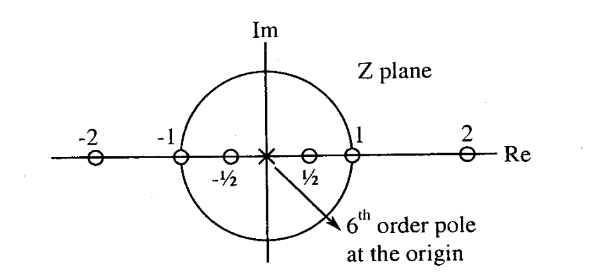
\includegraphics[width=0.6\textwidth]{2.png} 
      \caption{}
    \label{fig:fig2} 
\end{figure}
Which one of the following statements is TRUE?
\begin{multicols}{2}
\begin{enumerate}
\item This is a low pass filter
\item This is a high pass filter
\item This is an IIR filter
\item This is an FIR filter
\end{enumerate}
\end{multicols} \hfill(GATE IN 2011)

\item The continuous time signal $x(t) = \cos(100\pi t) + \sin(300\pi t)$ is sampled at the rate 100 Hz to get the signal
$x_s(t) = \sum_{n=-\infty}^{\infty} x(nT_s) \delta(t-nT_s), \quad T_s = \text{sampling period}$
The signal $x_s(t)$ is passed through an ideal low pass filter with cutoff frequency 100 Hz. The output of the filter is proportional to

\begin{multicols}{2}
\begin{enumerate}
\item $\cos(100\pi t)$
\item $\cos(100\pi t) + \sin(100\pi t)$
\item $\cos(100\pi t) - \sin(100\pi t)$
\item $\sin(100\pi t)$
\end{enumerate}
\end{multicols} \hfill(GATE IN 2011)

\item Consider a system with input $x(t)$ and output $y(t)$ related as follows
$y(t) = \frac{d}{dt} \left[ e^{-t} x(t) \right]$
Which one of the following statements is TRUE?

\begin{multicols}{2}
\begin{enumerate}
\item The system is nonlinear
\item The system is time-invariant
\item The system is stable
\item The system has memory
\end{enumerate}
\end{multicols} \hfill(GATE IN 2011)

\item The first two rows of Routh's table of a third-order characteristic equation are:
$
s^3 \quad 3 \quad 3 \\
s^2 \quad 4 \quad 4 \\
$
It can be inferred that the system has
\begin{enumerate}
\item One real pole in the right-half of s-plane
\item A pair of complex conjugate poles in the right-half of s-plane
\item A pair of real poles symmetrically placed around $ s = 0 $
\item A pair of complex conjugate poles on the imaginary axis of the s-plane
\end{enumerate}
\hfill(GATE IN 2011)
\item The amplifier shown has a voltage gain of -2.5, an input resistance of $10\,k\Omega$, and a lower 3-dB cut-off frequency of 20 Hz. Which one of the following statements is TRUE when the emitter resistance $ R_E $ is doubled?
\begin{figure}[H]
    \centering
      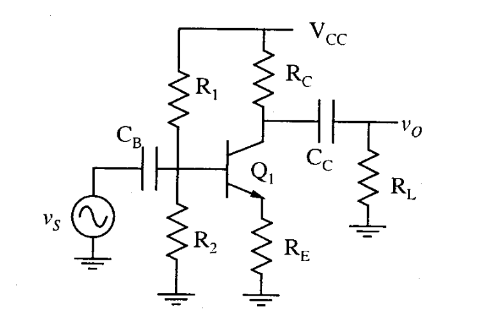
\includegraphics[width=0.6\textwidth]{3.png} 
      \caption{}
    \label{fig:fig3} 
\end{figure}
\begin{multicols}{2}
\begin{enumerate}
\item Magnitude of voltage gain will decrease  
\item Input resistance will decrease  
\item Collector bias current will increase  
\item Lower 3-dB cut-off frequency will increase
\end{enumerate}
\end{multicols} \hfill(GATE IN 2011)

\item Figure below shows a circuit for implementing an 8-bit Digital-to-Analog converter (DAC) using two identical 4-bit DACs with equal reference voltages. Assume that $b_0$ represents LSB, $b_7$ MSB and the opamp is ideal. To obtain correct analog values corresponding to an 8-bit DAC at the output $V_O$, the value of resistor $R$ is
\begin{figure}[H]
    \centering
      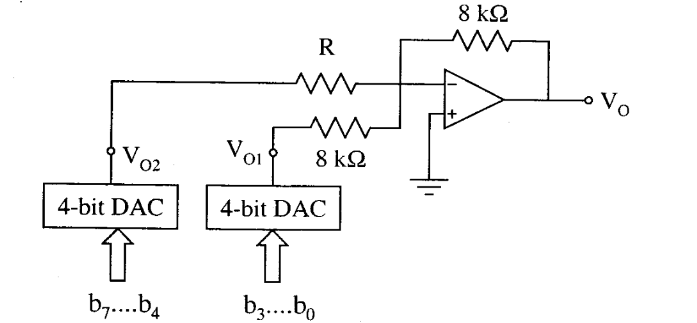
\includegraphics[width=0.6\textwidth]{4.png} 
      \caption{}
    \label{fig:fig4} 
\end{figure}
\begin{multicols}{4}
\begin{enumerate}
\item 0.25 k$\Omega$
\item 0.5 k$\Omega$
\item 1 k$\Omega$
\item 8 k$\Omega$
\end{enumerate}
\end{multicols} \hfill(GATE IN 2011)


\item In the circuit, the switch initially at position 1 for a long time is changed to position 2 at $ t = 0 $. The current $ i(t) $ through the inductor for $ t \geq 0 $ is
\begin{figure}[H]
    \centering
      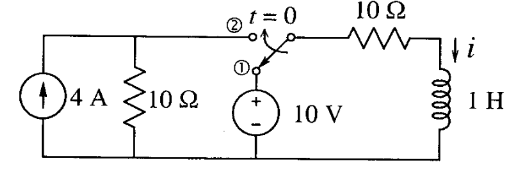
\includegraphics[width=0.6\textwidth]{5.png} 
      \caption{}
    \label{fig:fig5} 
\end{figure}
\begin{multicols}{2}
\begin{enumerate}
\item $1 - e^{-20t}\,A$  
\item $1 + e^{-20t}\,A$  
\item $1 + 2e^{-20t}\,A$  
\item $2 - e^{-20t}\,A$
\end{enumerate}
\end{multicols} \hfill(GATE IN 2011)

\item The current $ I $ shown in the circuit is equal to
\begin{figure}[H]
    \centering
      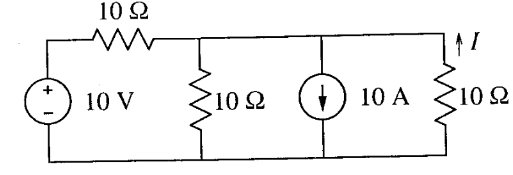
\includegraphics[width=0.6\textwidth]{6.png} 
      \caption{}
    \label{fig:fig6} 
\end{figure}
\begin{multicols}{4}
\begin{enumerate}
\item $3\,A$  
\item $3.67\,A$  
\item $6\,A$  
\item $9\,A$
\end{enumerate}
\end{multicols} \hfill(GATE IN 2011)

\item The transfer function $ \frac{C}{R} $ of the system represented by the signal flow graph is
\begin{figure}[H]
    \centering
      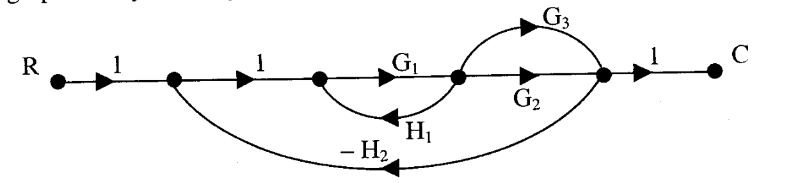
\includegraphics[width=0.6\textwidth]{7.png} 
      \caption{}
    \label{fig:fig7} 
\end{figure}
\begin{enumerate}
\item $ \frac{G_1G_2 + G_1G_3}{1 + G_1G_2H_2} $  
\item $ \frac{G_1G_2 + G_1G_3}{1 - G_1H_1 + G_1G_2H_2} $  
\item $ \frac{G_1G_2 + G_1G_3}{1 - G_1H_1 + G_1G_2H_2 + G_1G_3H_2} $  
\item $ \frac{G_1G_2 + G_1G_3}{1 - G_1H_1 + G_1G_2H_2 + G_1G_3H_2 + G_1G_2G_3H_1} $
\end{enumerate}
\hfill(GATE IN 2011)
\item For the Boolean expression $ f = |\overline{a}\overline{b}\overline{c} + \overline{a}b\overline{c} + \overline{a}\overline{b}c + a\overline{b}\overline{c} + abc $, the minimized Product of Sum (PoS) expression is
\begin{enumerate}
\item $ (b + \overline{c})(a + \overline{c}) $  
\item $ (\overline{b} + c)(\overline{a} + c) $  
\item $ (\overline{b} + c)(a + \overline{c}) $  
\item $ \overline{c} + abc $
\end{enumerate}
\hfill(GATE IN 2011)

\item The base of the number system for the addition operation $ 24 + 14 = 41 $ to be true is
\begin{multicols}{4}
\begin{enumerate}
\item 8  
\item 7  
\item 6  
\item 5
\end{enumerate}
\end{multicols} \hfill(GATE IN 2011)

\item An $8K \times 8$ bit RAM is interfaced to an 8085 microprocessor. In a fully decoded scheme, if the address of the last memory location is 4FFFH, the address of the first memory location of RAM is
\begin{multicols}{4}
\begin{enumerate}
\item 1000H  
\item 2000H  
\item 3000H  
\item 4000H
\end{enumerate}
\end{multicols} \hfill(GATE IN 2011)
\item The Treadmill Test is used to diagnose
\begin{enumerate}
\item The balancing style during walk of the patient  
\item The auditory activity of the patient  
\item The visual activity of the patient  
\item The cardiac activity of the patient
\end{enumerate}
\hfill(GATE IN 2011)
\item The characteristics of a thermometer measuring ambient temperature is $ 2\frac{dT_i}{dt} + T_i - T_a = 0 $, where $ T_i $ and $ T_a $ are indicated and ambient temperatures respectively,both in $\degree C$. The -3 dB cut-off frequency is
\begin{multicols}{4}
\begin{enumerate}
\item $\frac{1}{2}Hz$  
\item $ \frac{1}{4\pi}Hz $  
\item $1\,Hz$  
\item $2\pi\,Hz$
\end{enumerate}
\end{multicols} \hfill(GATE IN 2011)

\item For a copper-constantan (Type T) thermocouple, the junction potential $E$ (in $\mu$V) at $0^\circ$C is given by:  
$E = 38.740 + 3.3 \times 10^{-2} T^2 + 2.07 \times 10^{-4} T^3 - 2.2 \times 10^{-6} T^4 + \text{higher order terms}$  
Assuming cold junction compensation, the sensitivity of the thermocouple at $100^\circ$C is approximately:
\begin{multicols}{4}
\begin{enumerate}
\item 45.34 $\mu$V/$^\circ$C  
\item 42.75 $\mu$V/$^\circ$C  
\item 38.74 $\mu$V/$^\circ$C  
\item 0.06 $\mu$V/$^\circ$C
\end{enumerate}
\end{multicols} \hfill(GATE IN 2011)

\item A furnace temperature is monitored from 50 m away. The transmitter has a range of 0–500$^\circ$C and provides a 4–20 mA output. The temperature is determined from the voltage across a 500 $\Omega$ resistor in the loop. If the measured voltage is 4 V, the furnace temperature is:
\begin{multicols}{4}
\begin{enumerate}
\item 100 $^\circ$C  
\item 125 $^\circ$C  
\item 150 $^\circ$C  
\item 200 $^\circ$C
\end{enumerate}
\end{multicols} \hfill(GATE IN 2011)

\item The core/cladding index difference of a single-mode optical fiber is 0.01. The refractive index of the core material is 1.5. The maximum angle of acceptance of the fiber is approximately:
\begin{multicols}{4}
\begin{enumerate}
\item 17.5$^\circ$  
\item 12.1$^\circ$  
\item 8.6$^\circ$  
\item 2.0$^\circ$
\end{enumerate}
\end{multicols} \hfill(GATE IN 2011)

\item The conventional way of expressing vibration is in terms of:
\begin{multicols}{2}
\begin{enumerate}
\item Richter scale  
\item Acceleration due to gravity  
\item Speed of sound  
\item Atmospheric pressure
\end{enumerate}
\end{multicols} \hfill(GATE IN 2011)

\item The primary and secondary key of an LVDT (stroke length $\pm$50 mm) are connected to a 3 kHz sinusoidal source and a diode bridge-based phase-sensitive demodulator. The core remains static at 15 mm above the null position. The frequency of the voltage observed at the input of the low-pass filter is:
\begin{multicols}{4}
\begin{enumerate}
\item 1 kHz  
\item 1.5 kHz  
\item 3 kHz  
\item 6 kHz
\end{enumerate}
\end{multicols} \hfill(GATE IN 2011)

\item The series  
$\sum_{m=0}^{\infty} \frac{(x-1)^{2m}}{4^m}$  
converges for:
\begin{multicols}{4}
\begin{enumerate}
\item $-2 < x < 2$  
\item $-1 < x < 3$  
\item $-3 < x < 1$  
\item $x < 3$
\end{enumerate}
\end{multicols} \hfill(GATE IN 2011)

\item Consider the differential equation:  
$y'' + 2y' + y = 0,\quad y(0) = 1,\quad y(1) = 0$  
The value of $y(2)$ is:
\begin{multicols}{4}
\begin{enumerate}
\item $-1$  
\item $-e^{-1}$  
\item $-e^{-2}$  
\item $-e^{2}$
\end{enumerate}
\end{multicols} \hfill(GATE IN 2011)

\item Box 1 contains chips numbered 3, 6, 9, 12, 15. Box 2 contains chips numbered 6, 11, 16, 21, 26. One chip is drawn from each box and their numbers are multiplied. The probability that the product is even is:
\begin{multicols}{4}
\begin{enumerate}
\item $\frac{6}{25}$  
\item $\frac{2}{5}$  
\item $\frac{3}{5}$  
\item $\frac{19}{25}$
\end{enumerate}
\end{multicols} \hfill(GATE IN 2011)

\item The extremum (minimum or maximum) point of a function $f(x)$ is to be determined by solving $ \frac{d f(x)}{dx} = 0 $ using the Newton-Raphson method. Let $f(x) = x^3 - 6x$ and $x_0 = 1$ be the initial guess of $x$. The value of $x$ after two iterations ($x_2$) is

\begin{multicols}{4}
\begin{enumerate}
\item 0.0141
\item 1.4142
\item 1.4167
\item 1.5000
\end{enumerate}
\end{multicols} \hfill(GATE IN 2011)

\item The unit-step response of a negative unity feedback system with open-loop transfer function  
$G(s) = \frac{6}{s + 5}$  
is:
\begin{multicols}{4}
\begin{enumerate}
\item $1 - e^{-5t}$  
\item $6 - 6e^{-5t}$  
\item $\frac{6}{5} - \frac{6}{5}e^{-5t}$
\item $\frac{6}{11} - \frac{6}{11}e^{-5t}$
\end{enumerate}
\end{multicols} \hfill(GATE IN 2011)


\item The transfer function of the system described by the state-space equations $ \myvec{\dot{x}_1 \\ \dot{x}_2}=\myvec{-4 -1 \\-3 -1}\myvec{x_1 \\ x_2} +\myvec{1 \\ 1}u,\Vec{y}=\myvec{1 0}\myvec{x_1 \\ x_2}$ 
is 

\begin{multicols}{4}
\begin{enumerate}
\item $\frac{s}{s^2 + 5s + 1}$
\item $\frac{2s}{s^2 + 5s + 1}$
\item $\frac{3s}{s^2 + 5s + 1}$
\item $\frac{4s}{s^2 + 5s + 1}$
\end{enumerate}
\end{multicols} \hfill(GATE IN 2011)


\item Consider the second-order system with the characteristic equation  
$s(s + 3) + K(s + 5) = 0$  
The complex portion of the root locus for $0 < K < \infty$ lies on a circle. The two breakaway points on the real axis are:
\begin{multicols}{4}
\begin{enumerate}
\item $-5 \pm \dfrac{\sqrt{5}}{2}$  
\item $-5 \pm \sqrt{5}$  
\item $-5 \pm \sqrt{10}$  
\item $-5 \pm {2}\sqrt{5}$
\end{enumerate}
\end{multicols} \hfill(GATE IN 2011)

\item In a flapper-nozzle displacement transducer, the following parameters are given:  
Diameter of orifice = $0.2$ mm, Diameter of nozzle = $0.8$ mm, Supply pressure = $1.4 \times 10^2$ kPa (gauge), Ambient pressure = $0$ (gauge).  
The maximum value of sensitivity is:
\begin{multicols}{4}
\begin{enumerate}
\item $4.0$ MPa/mm  
\item $5.6$ MPa/mm  
\item $6.4$ MPa/mm  
\item $7.3$ MPa/mm
\end{enumerate}
\end{multicols} \hfill(GATE IN 2011)

\item A differential push-pull type capacitive displacement sensor (nominal capacitance $C_0 = 0.01\,\mu$F) is connected in two adjacent arms of an AC bridge in such a way that output voltage of bridge is independent of frequency of supply voltage. Supply to the bridge is $1$ V at $1$ kHz, and two equal resistances $R = 3.9$ k$\Omega$ are placed in the other arms. The bridge sensitivity is:
\begin{multicols}{4}
\begin{enumerate}
\item $0.001$ mV/pF  
\item $0.05$ mV/pF  
\item $0.1$ mV/pF  
\item $0.5$ mV/pF
\end{enumerate}
\end{multicols} \hfill(GATE IN 2011)

\item A turbine flowmeter is rotating at $72$ rpm. The flux $\Psi(\theta)$ linked to the nearby magnet and coil assembly is given by $\Psi(\theta) = 3 + \cos(4\theta)$ mWb, where $\theta$ is the angular position (in radians).  
The amplitude and frequency of the output voltage signal are:
\begin{multicols}{2}
\begin{enumerate}
\item $4$ mV and $45.8$ Hz  
\item $30.2$ mV and $4.8$ Hz  
\item $30.2$ mV and $30.2$ Hz  
\item $288$ mV and $45.8$ Hz
\end{enumerate}
\end{multicols} \hfill(GATE IN 2011)

\item Assuming base-emitter voltage of $0.7$ V and $\beta = 99$ for transistor $Q_1$, the output voltage $V_o$ in the ideal opamp circuit is:
\begin{figure}[H]
    \centering
      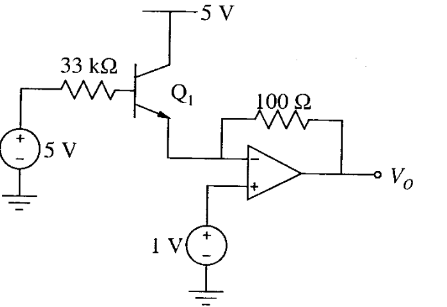
\includegraphics[width=0.6\textwidth]{8.png} 
      \caption{}
    \label{fig:fig8} 
\end{figure}
\begin{multicols}{4}
\begin{enumerate}
\item $-1$ V  
\item $-\dfrac{1}{3.3}$ V  
\item $0$ V  
\item $2$ V
\end{enumerate}
\end{multicols} \hfill(GATE IN 2011)

\item Assuming zener diode $D_1$ has the I-V characteristics shown and forward voltage drop of diode $D_2$ is $0.7$ V, the voltage $V_o$ in the circuit is:
\begin{multicols}{2}
\begin{figure}[H]
      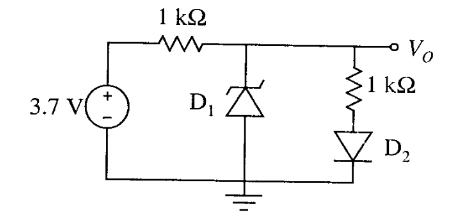
\includegraphics[width=0.3\textwidth]{9.png} 
      \caption{}
    \label{fig:fig9} 
\end{figure}
\begin{figure}[H]
      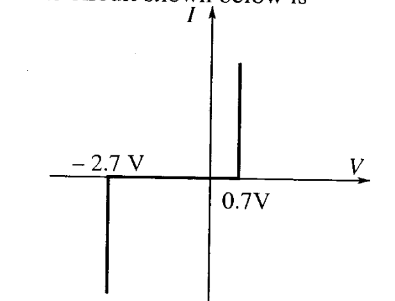
\includegraphics[width=0.3\textwidth]{10.png} 
      \caption{}
    \label{fig:fig10} 
\end{figure}
\end{multicols}
\begin{multicols}{4}
\begin{enumerate}
\item $3.7$ V  
\item $2.7$ V  
\item $2.2$ V  
\item $0$ V
\end{enumerate}
\end{multicols} \hfill(GATE IN 2011)

\item The transfer characteristics of the circuit are observed on an oscilloscope in XY mode. $V_i$ is connected to X input (0.5 V/div), $V_o$ to Y input (2 V/div). The beam is at origin when $V_i = 0$. 
\begin{multicols}{2}
\begin{figure}[H]
      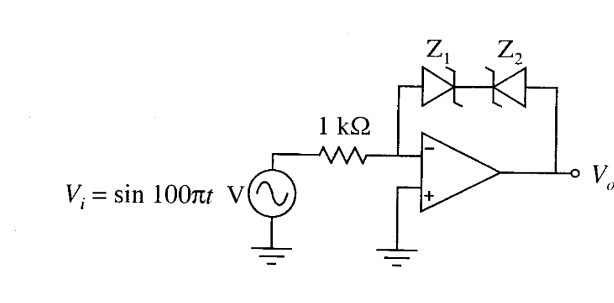
\includegraphics[width=0.3\textwidth]{11.png} 
      \caption{}
    \label{fig:fig11} 
\end{figure}
\begin{figure}[H]
      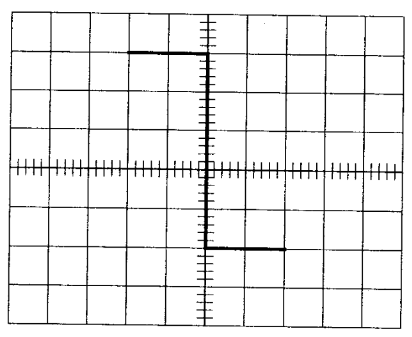
\includegraphics[width=0.3\textwidth]{12.png} 
      \caption{}
    \label{fig:fig12} 
\end{figure}
\end{multicols}
Assuming ideal opamp and zener diodes with $0.7$ V forward drop, the reverse breakdown voltages of $Z_1$ and $Z_2$ are:
\begin{multicols}{4}
\begin{enumerate}
\item $3.3$ V and $5.3$ V  
\item $4.7$ V and $6.7$ V  
\item $6.7$ V and $4.7$ V  
\item $5.3$ V and $3.3$ V
\end{enumerate}
\end{multicols} \hfill(GATE IN 2011)

\item Power in a three-phase star-connected balanced inductive load is measured by two-wattmeter method. Phase voltage = $230$ V, Phase current = $5$ A, Power factor = $0.707$.  
The readings $P_1$ and $P_2$ of the two wattmeters are:
\begin{multicols}{2}
\begin{enumerate}
\item $P_1 = 298$ W, $P_2 = 1111$ W  
\item $P_1 = 516$ W, $P_2 = 1924$ W  
\item $P_1 = 1220$ W, $P_2 = 1220$ W  
\item $P_1 = 1111$ W, $P_2 = -516$ W
\end{enumerate}
\end{multicols} \hfill(GATE IN 2011)

\item In the Wheatstone bridge shown, when resistance $R_1$ increases by $1\,\Omega$, the current through the galvanometer is:
\begin{figure}[H]
    \centering
      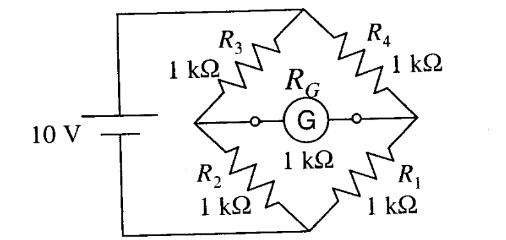
\includegraphics[width=0.6\textwidth]{13.png} 
      \caption{}
    \label{fig:fig13} 
\end{figure}
(consider the Thevenin equivalent resistance of the bridge in the calculations)
\begin{multicols}{4}
\begin{enumerate}
\item $1.25\,\mu$A  
\item $2.5\,\mu$A  
\item $12.5\,\mu$A  
\item $25\,\mu$A
\end{enumerate}
\end{multicols} \hfill(GATE IN 2011)


\item The value of $V_o$ of the series regulator shown below is:
\begin{figure}[H]
    \centering
      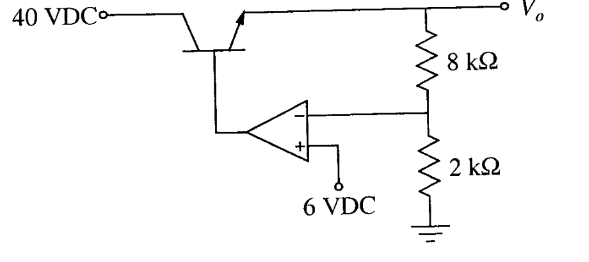
\includegraphics[width=0.6\textwidth]{14.png} 
      \caption{}
    \label{fig:fig14} 
\end{figure}
\begin{multicols}{4}
\begin{enumerate}
\item $24$ V  
\item $28$ V  
\item $30$ V  
\item $32$ V
\end{enumerate}
\end{multicols} \hfill(GATE IN 2011)

\item The ideal opamp-based circuit shown below acts as a:
\begin{figure}[H]
    \centering
      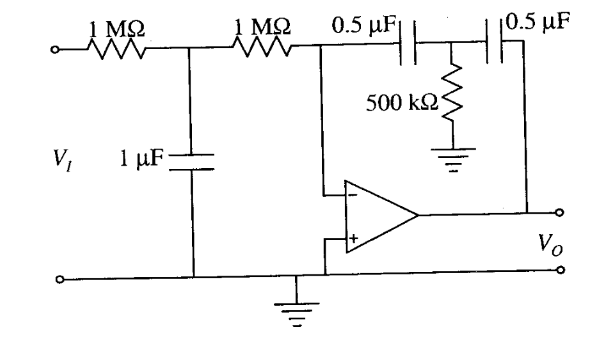
\includegraphics[width=0.6\textwidth]{15.png} 
      \caption{}
    \label{fig:fig15} 
\end{figure}
\begin{multicols}{4}
\begin{enumerate}
\item Low-pass filter  
\item High-pass filter  
\item Band-pass filter  
\item Band-reject filter
\end{enumerate}
\end{multicols} \hfill(GATE IN 2011)

\item A $4$-bit successive approximation type of A/D converter has an input range of $0$ to $15$ volts. The output bit $b_1$ next to the LSB has a stuck-at-zero fault. The pair of input voltages that produces the same output code word is:
\begin{multicols}{4}
\begin{enumerate}
\item $2$ V and $4$ V  
\item $4$ V and $6$ V  
\item $1$ V and $2$ V  
\item $8$ V and $9$ V
\end{enumerate}
\end{multicols} \hfill(GATE IN 2011)

\item The number of objects crossing a window sequentially at variable speed is to be counted using an interrupt in the $8085$ microprocessor. The objects are sensed by an optical source and detector. The output is logic high while the object is in front of the window and this output is used to interrupt the detector. The duration ranges from $100$ ms to $2$ s. The processor takes $1$ ms to process the input. The best choice of interrupt for error-free counting is:
\begin{multicols}{4}
\begin{enumerate}
\item RST $5.5$  
\item RST $6.5$  
\item RST $7.5$  
\item INTR
\end{enumerate}
\end{multicols} \hfill(GATE IN 2011)

\item The circuit below shows an up/down counter working with a decoder and a flip-flop.Preset and Clear of the flip-flop are asynchronous active-low inputs.Assuming that the initial value of counter output ($Q_2 Q_1 Q_0$) as zero,the counter outputs in decimal for 12 clock cycles are
\begin{figure}[H]
    \centering
      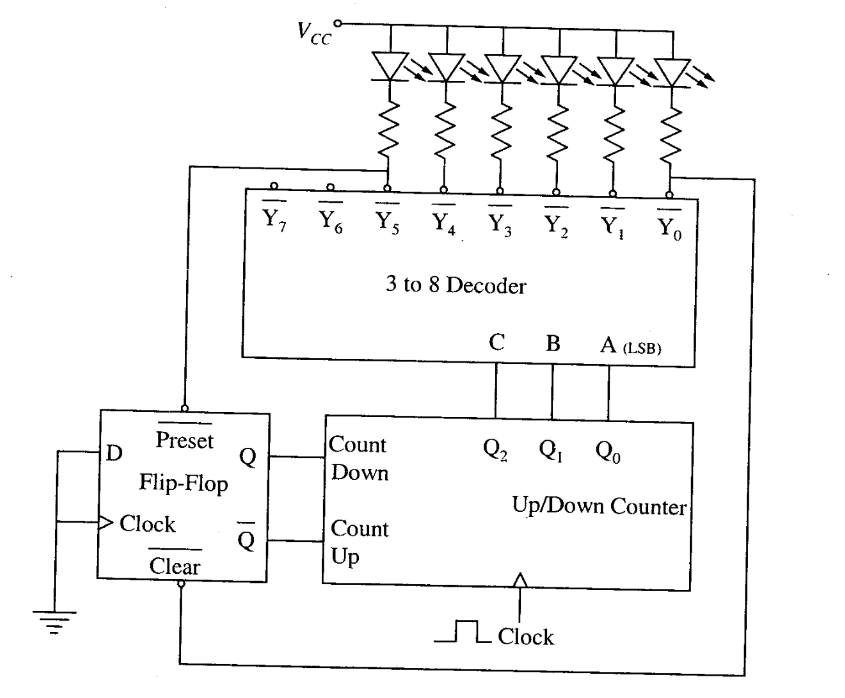
\includegraphics[width=0.6\textwidth]{16.png} 
      \caption{}
    \label{fig:fig16} 
\end{figure}
\begin{enumerate}
\item 0,1,2,3,4,4,3,2,1,1,2,3,4
\item 0,1,2,3,4,5,0,1,2,3,4,5,0
\item 0,1,2,3,4,5,5,4,3,2,1,0,1
\item 0,1,2,3,4,5,4,3,2,1,0,1,2
\end{enumerate}
 \hfill(GATE IN 2011)

\item A square wave (amplitude $\pm 10$ mV, frequency $5$ kHz, duty cycle $50\%$) is passed through an ideal low-pass filter with $0$ dB gain and cutoff frequency $10$ kHz. The filtered signal is buried in zero-mean noise with one-sided PSD of $25$ pW/Hz up to $2$ MHz. The signal-to-noise ratio of the output is:
\begin{multicols}{4}
\begin{enumerate}
\item $0$ dB  
\item $0.1$ dB  
\item $1.0$ dB  
\item $3$ dB
\end{enumerate}
\end{multicols} \hfill(GATE IN 2011)

\item Consider the difference equation $y[n] - \frac{1}{3} y[n-1] = x[n]$ and suppose that $x[n] = \left( \frac{1}{2} \right)^n u[n]$. Assuming the condition of initial rest, the solution for $y[n]$, $n \geq 0$ is

\begin{multicols}{4}
\begin{enumerate}
\item $3 \left( \frac{1}{3} \right)^n - 2 \left( \frac{1}{2} \right)^n$
\item $-2 \left( \frac{1}{3} \right)^n + 3 \left( \frac{1}{2} \right)^n$
\item $\frac{2}{3} \left( \frac{1}{3} \right)^n + \frac{1}{3} \left( \frac{1}{2} \right)^n$
\item $\frac{1}{3} \left( \frac{1}{3} \right)^n + \frac{2}{3} \left( \frac{1}{2} \right)^n$
\end{enumerate}
\end{multicols} \hfill(GATE IN 2011)

\textbf{Common Data Questions}\\
\textbf{Common Data for Q48 and Q49}
 Consider the circuit given below
 \begin{figure}[H]
    \centering
      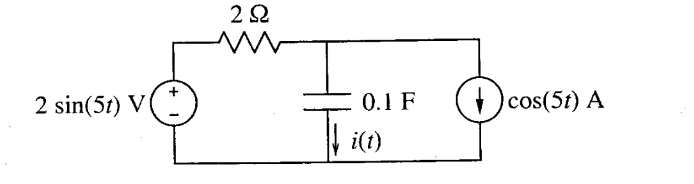
\includegraphics[width=0.6\textwidth]{17.png} 
      \caption{}
    \label{fig:fig17} 
\end{figure}
\item The current $i(t)$ through the capacitor is:
\begin{multicols}{4}
\begin{enumerate}
\item $\sin(5t)$ A  
\item $\cos(5t)$ A  
\item $\sin(5t - 45^\circ)$ A  
\item $1$ A
\end{enumerate}
\end{multicols} \hfill(GATE IN 2011)

\item The average total power delivered by the two sources in the above circuit is:
\begin{multicols}{4}
\begin{enumerate}
\item $0$ W  
\item $0.5$ W  
\item $2$ W  
\item $4$ W
\end{enumerate}
\end{multicols} \hfill(GATE IN 2011)

\textbf{Common Data for Q50 and Q51}
The open-loop transfer function of a unity negative feedback control system is given by  
$G(s) = \dfrac{K(s+5)^3}{s^3}$  
\item The value of $K$ for the phase margin of the system to be $45^\circ$ is:
\begin{multicols}{4}
\begin{enumerate}
\item $250\sqrt{5}$  
\item $250\sqrt{2}$  
\item $125\sqrt{5}$  
\item $125\sqrt{2}$
\end{enumerate}
\end{multicols} \hfill(GATE IN 2011)

\item For the same system, the value of $K$ for the damping ratio $\zeta = 0.5$ corresponding to the dominant closed-loop complex conjugate pole pair is:
\begin{multicols}{4}
\begin{enumerate}
\item $250$  
\item $125$  
\item $75$  
\item $50$
\end{enumerate}
\end{multicols} \hfill(GATE IN 2011)

\textbf{Common Data for Q52 and Q53}
The level of water, stored in a truncated conical bath, is measured by a gamma-ray radiation sensor. The initial level of water is 1 m, and the level is increasing due to water inflow at the constant rate of $0.125m^3/s$. Assume mass absorption coefficient of water is $77 \times 10^{-4}  m^2/kg$ and density of water is $1000  kg/m^3$.
\begin{figure}[H]
    \centering
      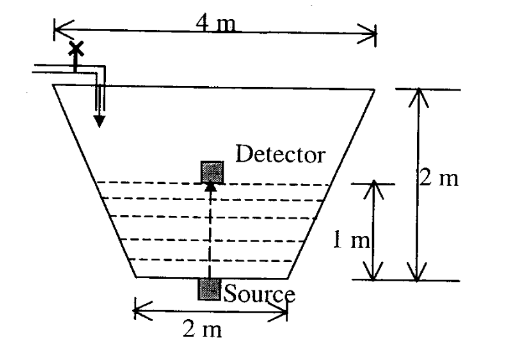
\includegraphics[width=0.6\textwidth]{18.png} 
      \caption{}
    \label{fig:fig18} 
\end{figure}

\item When the intensity of radiation received by the floating detector is half of the intensity detected initially, the level of water is

\begin{multicols}{4}
\begin{enumerate}
\item 1.09 m
\item 1.5 m
\item 1.8 m
\item 1.9 m
\end{enumerate}
\end{multicols} \hfill(GATE IN 2011)

\item When the floating detector is at the level calculated in Q.52, the time elapsed is

\begin{multicols}{4}
\begin{enumerate}
\item 4.1 s
\item 5.23 s
\item 10.52 s
\item 50.63 s
\end{enumerate}
\end{multicols} \hfill(GATE IN 2011)

\textbf{Common Data for Q54 and Q55}
M1, M2 and M3 in the circuit shown below are matched N-channel enhancement mode MOSFETs operating in saturation mode, forward voltage drop of each diode is 0.7 V, reverse leakage current of each diode is negligible and the opamp is ideal.
\begin{figure}[H]
    \centering
      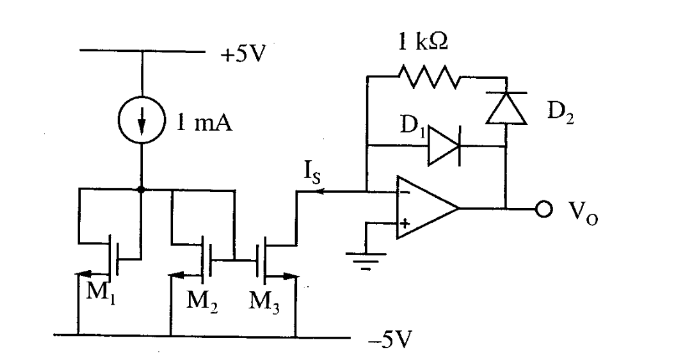
\includegraphics[width=0.6\textwidth]{19.png} 
      \caption{}
    \label{fig:fig19} 
\end{figure}

\item The current $I_S$ in the circuit is

\begin{multicols}{4}
\begin{enumerate}
\item $-1$ mA
\item 0.5 mA
\item 1 mA
\item 2 mA
\end{enumerate}
\end{multicols} \hfill(GATE IN 2011)

\item For the computed value of current $I_S$, the output voltage $V_O$ is

\begin{multicols}{4}
\begin{enumerate}
\item 1.2 V
\item 0.7 V
\item 0.2 V
\item $-0.7$ V
\end{enumerate}
\end{multicols} \hfill(GATE IN 2011)
\textbf{General Aptitude (GA) Questions}
\item There are two candidates P and Q in an election. During the campaign, 40\% of the voters promised to vote for P, and rest for Q. However, on the day of election 15\% of the voters went back on their promise to vote for P and instead voted for Q. 25\% of the voters went back on their promise to vote for Q and instead voted for P. Suppose, P lost by 2 votes, then what was the total number of voters?

\begin{multicols}{4}
\begin{enumerate}
\item 100
\item 110
\item 90
\item 95
\end{enumerate}
\end{multicols} \hfill(GATE IN 2011)

\item The question below consists of a pair of related words followed by four pairs of words. Select the pair that best expresses the relation in the original pair:

Gladiator : Arena

\begin{enumerate}
\item dancer : stage
\item commuter : train
\item teacher : classroom
\item lawyer : courtroom
\end{enumerate}
\hfill(GATE IN 2011)

\item Choose the most appropriate word from the options given below to complete the following sentence:

\textbf{Under ethical guidelines recently adopted by the Indian Medical Association, human genes are to be manipulated only to correct diseases for which \_\_\_\_\_\_\_ treatments are unsatisfactory.}


\begin{enumerate}
\item similar
\item most
\item uncommon
\item available
\end{enumerate}
\hfill(GATE IN 2011)

\item Choose the word from the options given below that is most nearly opposite in meaning to the given word:

\textbf{Frequency}


\begin{enumerate}
\item periodicity
\item rarity
\item gradualness
\item persistency
\end{enumerate}
\hfill(GATE IN 2011)

\item Choose the most appropriate word from the options given below to complete the following sentence:

\textbf{It was her view that the country's problems had been \_\_\_\_\_\_\_ by foreign technocrats, so that to invite them to come back would be counter-productive.}


\begin{enumerate}
\item identified
\item ascertained
\item exacerbated
\item analysed
\end{enumerate}
 \hfill(GATE IN 2011)

\item The fuel consumed by a motorcycle during a journey while traveling at various speeds is indicated in the graph below.
\begin{figure}[H]
    \centering
      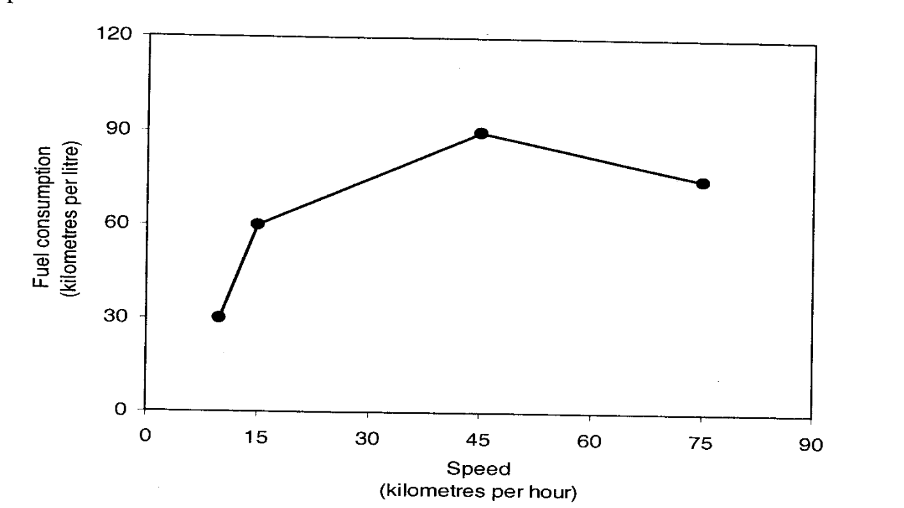
\includegraphics[width=0.6\textwidth]{20.png} 
      \caption{}
    \label{fig:fig20} 
\end{figure}
The distances covered during four laps of the journey are listed in the table below


\begin{table}[H]
\begin{tabular}{|c|c|c|}
\hline
Lap & Distance (kilometres) & Average speed (kilometres per hour) \\
\hline
P & 15 & 15 \\
Q & 75 & 45 \\
R & 40 & 75 \\
S & 10 & 10 \\
\hline
\end{tabular}
\caption{}
\label{tab:tab1}
\end{table}


From the given data, we can conclude that the fuel consumed per kilometre was least during the lap

\begin{multicols}{4}
\begin{enumerate}
\item P
\item Q
\item R
\item S
\end{enumerate}
\end{multicols} \hfill(GATE IN 2011)

\item \textbf{The horse has played a little known but very important role in the field of medicine. Horses were injected with toxins of diseases until their blood built up immunities. Then a serum was made from their blood. Serums to fight with diphtheria and tetanus were developed this way. It can be inferred from the passage, that horses were}


\begin{enumerate}
\item given immunity to diseases
\item generally quite immune to diseases
\item given medicines to fight toxins
\item given diphtheria and tetanus serums
\end{enumerate}
 \hfill(GATE IN 2011)

\item The sum of $n$ terms of the series $4+44+444+\ldots$ is


\begin{enumerate}
\item $\frac{4}{81} [10^{n+1}-9n-1]$
\item $\frac{4}{81} [10^{n-1}-9n-1]$
\item $\frac{4}{81} [10^{n+1}-9n-10]$
\item $\frac{4}{81} [10^{n}-9n-10]$
\end{enumerate}
 \hfill(GATE IN 2011)

\item Given that $f(y)=|y| / y$, and $q$ is any non-zero real number, the value of $|f(q)-f(-q)|$ is

\begin{multicols}{4}
\begin{enumerate}
\item 0
\item $-1$
\item 1
\item 2
\end{enumerate}
\end{multicols} \hfill(GATE IN 2011)

\item Three friends, R, S and T shared toffee from a bowl. R took $1/3^{rd}$ of the toffees, but returned four to the bowl. S took $1/4^{th}$ of what was left but returned three toffees to the bowl. T took half of the remainder but returned two back into the bowl. If the bowl had 17 toffees left, how many toffees were originally there in the bowl?

\begin{multicols}{4}
\begin{enumerate}
\item 38
\item 31
\item 48
\item 41
\end{enumerate}
\end{multicols} 
\hfill(GATE IN 2011)
\end{enumerate}
\end{document}